%documentclass{beamer}
\documentclass[xcolor=dvipsnames]{beamer}
\usepackage{BioconductorSlides}
\usepackage{hyperref}
\usepackage[utf8]{inputenc}
%\usepackage[T1]{fontenc}
\usepackage{amsmath,amssymb,amsfonts,textcomp,setspace,graphicx,tikz,color}
\usepackage[absolute,overlay]{textpos}
\setlength{\TPHorizModule}{1mm}
\setlength{\TPVertModule}{1mm}

%\newcommand{\R}{{\texttt{R}}{}}

%%%%%%%%%%%%%%%%%%%%%%%%%%%%%%%%%%%%%%%%%%%%%%%%%%%%%%%%%%%%%%
%%%%%%%%%%%%   MODIFICAR AQUESTA SECCIÓ      %%%%%%%%%%%%%%%%%
%%%%%%%%%%%%%%%%%%%%%%%%%%%%%%%%%%%%%%%%%%%%%%%%%%%%%%%%%%%%%%
\title{Introduction to R and Bioconductor}
\author{Alex S\'anchez}
\institute[UEB]{Unitat d'Estadística i Bioinformàtica (UEB)}
\date{\today}
%%%%%%%%%%%%%%%%%%%%%%%%%%%%%%%%%%%%%%%%%%%%%%%%%%%%%%%%%%%%%%
%%%%%%%%%%%%%%%%%%%%%%%%%%%%%%%%%%%%%%%%%%%%%%%%%%%%%%%%%%%%%%
%%%%%%%%%%%%%%%%%%%%%%%%%%%%%%%%%%%%%%%%%%%%%%%%%%%%%%%%%%%%%%
%\setheme{BioconductorSlides}

%itemize
\newcommand{\bfr}{\begin{frame}}
\newcommand{\efr}{\end{frame}}
\newcommand{\ft}{\frametitle}


%itemize
\newcommand{\bit}{\begin{itemize}}
\newcommand{\eit}{\end{itemize}}

%enumerate
\newcommand{\ben}{\begin{enumerate}}
\newcommand{\een}{\end{enumerate}}

%Blue box
\newcommand{\bB}[1]{\begin{problock}{#1}}
\newcommand{\eB}{\end{problock}}

%Green box
\newcommand{\bG}[1]{\begin{exampleblock}{#1}}
\newcommand{\eG}{\end{exampleblock}}

%Red box
\newcommand{\bR}[1]{\begin{alertblock}{#1}}
\newcommand{\eR}{\end{alertblock}}

%colors
\definecolor{dB}{RGB}{80,13,138}
\definecolor{lB}{RGB}{153,0,153}

\definecolor{dG}{rgb}{0.00,0.50,0.00}
\definecolor{lG}{rgb}{0.71,0.81,0.69}

%custom blocks

\newenvironment<>{problock}[1]{%
  \begin{actionenv}#2%
      \def\insertblocktitle{#1}%
      \par%
      \mode<presentation>{%
       \setbeamercolor{block title}{fg=white,bg=Plum}
       \setbeamercolor{block body}{fg=black,bg=lightpurple}
       \setbeamercolor{itemize item}{fg=Plum}
       \setbeamertemplate{itemize item}[triangle]
     }%
      \usebeamertemplate{block begin}}
    {\par\usebeamertemplate{block end}\end{actionenv}}



\begin{document}

\begin{frame}[plain]
%\addtocounter{totalframenumber}{-1}
\titlepage
\end{frame}

\begin{frame}[Frame 1]
\addtocounter{framenumber}{-1}
\frametitle{Table of Contents}
\tableofcontents
\end{frame}

%%%%%%%%%%%%%%%%%%%%%%%%%%%%%%%%%%%%%%%%%%%%%%%%%%%%%%%%%%%%%%%%%%%%%%%%%
%%%%%%%%%%%%      MODIFICAR A PARTIR D'AQUI       %%%%%%%%%%%%%%%%%%%%%%%
%%%%%%%%%%%%%%%%%%%%%%%%%%%%%%%%%%%%%%%%%%%%%%%%%%%%%%%%%%%%%%%%%%%%%%%%%

\section{Objectives}

  \begin{frame}
   \frametitle{A bit of interaction}
    %\bB{The \textbf{\emph{main objective}} is...}
     %   to find differentially expressed genes (DEG) associated with Inflammatory Bowel 
      %  Disease (IBD) between samples of different tissues from bowels infected with three 
       % types of bacteria and a reference control
    %\eB
    
    \bit
      \item What is your R knowledge, on a 0(beginner) to 2 (expert) scale?
      \item How deep is your knowledge with R packages related 
	      			to NGS, on a 0(none) to 2 (good)scale?
      \item What analyses do you plan to do in R?
    \eit
\end{frame}

 \begin{frame}
\frametitle {Objectives}
\bit
\item Quick review of \R\, history and capabilities
\item Overview of the Bioconductor project
\item Bioconductor classes and methods for NGS
\eit
\end{frame}

\section{Introduction to R}
 \begin{frame}
  \frametitle{What is R?}
    \ben
    \item an implementation of the S language \tiny{(Bell Laboratories,Rick Becker, John Chambers and Allan Wilks)}
      \normalsize {
      \item R is an integrated suite of software for}
      		\bit
      			\item data manipulation
      			\item calculation and
      			\item graphical display.
      		\eit
    \een
  \end{frame}

   \begin{frame}
   \frametitle{What is R?(c'ed)}
	
    \ben
      \item R is a vehicle for newly developing methods of interactive data analysis
 
      		\bit
      			\item devolops rapidly
      			\item is being extenden by a large collection of packages
			    \bit
				\item Comprehensive R Archive Network (CRAN)
				\item Bioconductor
			    \eit
      			
      		\eit
      	\item However, most programs written in R are essentially ephimeral, written for a single piece of data analysis
    \een
  \end{frame}
  
 

   \begin{frame}
   \frametitle{R specifics}
	
    \bit
      \item a suite of operators for calculations on arrays, in particular matrices.
      \item an ``environment'':
      		\bit
      			\item a fully planned and coherent system,
      			\item it can be \emph{saved}, \emph{loaded}, \emph{exchanged}.
      		\eit
    \eit
  \end{frame}
  
  \begin{frame}
  \frametitle{R and statistics}
   \bit
      \item R is an environment...
	  \bit
	    \item originally not designed for statistics,
	    \item many classical and modern statistical techiniques implemented,
	  \eit 
\item Difference with S, S-plus, SAS or SPSS...
	  \bit
	    \item minimal ouput
	    \item minimal number of object (in comparison with the).
	  \eit
      \eit
     \end{frame}

   
     \begin{frame}
     \frametitle{R and the window system}
      \bit
	\item R comes with a graphical system on all plataform
	  \bit
	    \item console like: Unix
	    \item GUI and console: Mac, Windows
	  \eit
	 \item Integrated Developer Interfaces (IDE) have been developed
	 \bit
	    \item StatET plugin ( \url{http://www.walware.de/goto/statet}) for eclipse
	    \item \textbf{Rstudio} (\url{http://rstudio.org})
	 \eit
      \eit
      
     \end{frame}
     
        \begin{frame}
     \frametitle{Using R interactively}
      \bit
      \item Most of the time R is used interactively
	  \item R console is vey similar to Unix/linux
	    \bit
		\item \texttt{ls} command for listing,...
		\item The syntax is only slightly different:
		  \bit
		      \item \texttt{ls()} instead of \texttt{ls}
		  \eit
	    \eit
	   \item Documentation and help pages always avaliable:
	    \bit
		\item through the ``?'' command (\emph{perfect match})
		\item through the ``?'' command (\emph{fuzzy matching})
		\item through \texttt{help.start()} if you have a windows system
		\item searchable through \texttt{help.search()}
	    \eit
	  
      \eit
     \end{frame}

          \begin{frame}
     \frametitle{CRAN}
      \bit
          \item \url{http://cran.r-project.org}
	  \item The comprehensive R Archive
	    \bit
		\item 5578 packages! (26 May 2014)
		\item easy to install
		  \bit
		      \item R CMD INSTALL (cmd line)
		      \item \texttt{install.packages()} (from within the environment
		  \eit
	    \eit
      \eit
     \end{frame}
     
     
  \section{Bioconductor}

 \begin{frame}
     \frametitle{What is Bioconductor}
    \bit
    \item A software project for the analysis of genomic data
    \item \textbf{Open} source and \textbf{open} development.
    \item \url{http://bioconductor.org}
    \item A collection of R packages with \emph{some} common structures
	    \bit
		\item >1.100 packages (554 soft.,600 annot.)
		\item >300 developers, >4.000 citations
	    \eit
    \item Gentleman et al. \emph{Bioconductor: open software development for computational biology and bioinformatics}. Genome Biology (2004) vol. 5 (10) pp. R80
      \eit
     \end{frame}
 
  \begin{frame}
     \frametitle{Bioconductor: history and overview}
      \bit
    \item  Started in Harvard (2001) now hosted at Fred Hutchinson Cancer Research Center (FHCRC)
     \item Gentleman et al. \emph{Bioconductor: open software development for computational biology and bioinformatics}. Genome Biology (2004) vol. 5 (10) pp. R80
   \item Focus on \textbf{Microarray} at first, 
   \item and on \textbf{Next Generation Sequencing} as of 2008.
     \eit
    \end{frame}
     
    \begin{frame}
\frametitle{Bioconductor goals}
      \begin{itemize}
      \item Provide access to powerful\textbf{ statistical and graphical methods} for the analysis of biomedical and genomic data
      \item Facilitate the integration of \textbf{biological metadata} from WWW in the analysis of experimental data (e.g., GenBank, GO, LocusLink, PubMed)
      \item Allow the rapid development of \textbf{extensible, interoperable and scalable} software
      \item Promote \textbf{high-quality documentation} and \textbf{reproducible research}
      \item Provide \textbf{training} in computational and statistical methods
      \end{itemize}
    \end{frame}
  
     \begin{frame}
     \frametitle{FHCRC,BIOC core packages}
      \bit
	  \item Input and Output
	    \bit
		\item rtacklayer, \textbf{Rsamtools, ShortRead}
	    \eit
	  \item Sequence manipulation
	    \bit
		\item \textbf{Biostrings}
	    \eit
	  \item Range-based manipulations:
	    \bit
		\item \textbf{IRanges, GenomicRanges}
	    \eit
	  \item Annotations
	    \bit
		\item \textbf{GenomicFeatures}, AnnotationDbi, BSgenome
	    \eit
      \eit
     \end{frame}
     
       \begin{frame}
     \frametitle{}
     \begin{figure}[ht]
\centering
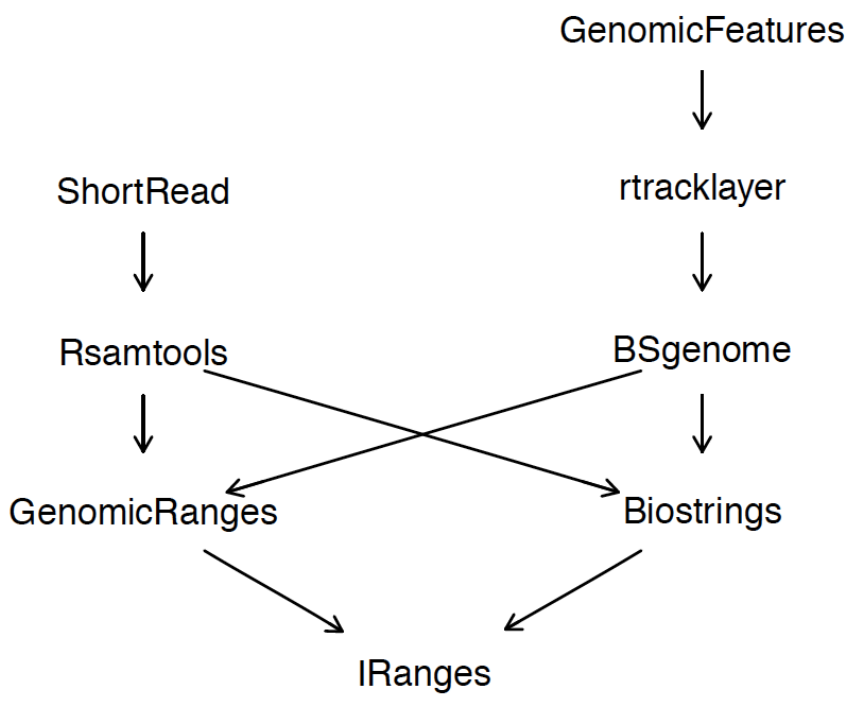
\includegraphics[width=80mm]{diagramas/Seleccio_001.png}
\end{figure}
     \end{frame}
    
       
     
      \begin{frame}{titre}
      \frametitle{53 Contributed packages (Sep. 2012)}
  \begin{columns}%
  
  
    \begin{column}[t]{0.45\textwidth}%
     \begin{itemize}
     \item Chip-seq(14)
      \begin{itemize}
        \item BayesPeak, CSAR, ChIPpeakAnno, ChiPseqR, ChIPsim, PICS, chipseq,...\\   
      \end{itemize}
     \item RNA-seq(18)
       \begin{itemize}
       \item DEGseq, DESeq, Genominator, baySeq, edgeR, srnaSeqMao, goseq, gage, easyRNASeq,..
      \end{itemize}
      \end{itemize}
    \end{column}
    
   
    \begin{column}[t]{0.45\textwidth}%
      \begin{itemize}
      \item \textbf{Infrastructure}: genomeIntervals, girafe, cqn
        \item \textbf{base calling}: Rolexa
        \item \textbf{Visualization}: HilbertVis, HilbertVisGUI
        \item \textbf{motif:} MotIV, rGADEM
        \item \textbf{domain-specific}: MEDIPS, OTUbase, R453Plus1Toolbox
        \item \textbf{database}: SRAdb, oneChannelGUI
        \item \textbf{smRNA}: segmentSeq
      \end{itemize}
    \end{column}
  \end{columns}
\end{frame}

\begin{frame}
 \frametitle{Installation}
  Two step installation
  \begin{itemize}
  \item First install R software: download from CRAN\\
\texttt{(www.cran.r-project.org)}
\item Install bioconductor
  \begin{itemize}
  \item Download installer from Bioconductor website \\
\texttt{> source("http://bioconductor.org/biocLite.R")}\\
\item Make default installation (installs some basic and some popular packages)\\
\texttt{> biocLite()}\\
\item Add what you specifically need\\
 \texttt{> biocLite(goProfiles)}
  \end{itemize}
 \end{itemize}
\end{frame}


     


\end{document}